% Options for packages loaded elsewhere
\PassOptionsToPackage{unicode}{hyperref}
\PassOptionsToPackage{hyphens}{url}
\PassOptionsToPackage{dvipsnames,svgnames,x11names}{xcolor}
%
\documentclass[
]{article}
\usepackage{amsmath,amssymb}
\usepackage{lmodern}
\usepackage{iftex}
\ifPDFTeX
  \usepackage[T1]{fontenc}
  \usepackage[utf8]{inputenc}
  \usepackage{textcomp} % provide euro and other symbols
\else % if luatex or xetex
  \usepackage{unicode-math}
  \defaultfontfeatures{Scale=MatchLowercase}
  \defaultfontfeatures[\rmfamily]{Ligatures=TeX,Scale=1}
\fi
% Use upquote if available, for straight quotes in verbatim environments
\IfFileExists{upquote.sty}{\usepackage{upquote}}{}
\IfFileExists{microtype.sty}{% use microtype if available
  \usepackage[]{microtype}
  \UseMicrotypeSet[protrusion]{basicmath} % disable protrusion for tt fonts
}{}
\makeatletter
\@ifundefined{KOMAClassName}{% if non-KOMA class
  \IfFileExists{parskip.sty}{%
    \usepackage{parskip}
  }{% else
    \setlength{\parindent}{0pt}
    \setlength{\parskip}{6pt plus 2pt minus 1pt}}
}{% if KOMA class
  \KOMAoptions{parskip=half}}
\makeatother
\usepackage{xcolor}
\usepackage[margin=1in]{geometry}
\usepackage{color}
\usepackage{fancyvrb}
\newcommand{\VerbBar}{|}
\newcommand{\VERB}{\Verb[commandchars=\\\{\}]}
\DefineVerbatimEnvironment{Highlighting}{Verbatim}{commandchars=\\\{\}}
% Add ',fontsize=\small' for more characters per line
\usepackage{framed}
\definecolor{shadecolor}{RGB}{248,248,248}
\newenvironment{Shaded}{\begin{snugshade}}{\end{snugshade}}
\newcommand{\AlertTok}[1]{\textcolor[rgb]{0.94,0.16,0.16}{#1}}
\newcommand{\AnnotationTok}[1]{\textcolor[rgb]{0.56,0.35,0.01}{\textbf{\textit{#1}}}}
\newcommand{\AttributeTok}[1]{\textcolor[rgb]{0.77,0.63,0.00}{#1}}
\newcommand{\BaseNTok}[1]{\textcolor[rgb]{0.00,0.00,0.81}{#1}}
\newcommand{\BuiltInTok}[1]{#1}
\newcommand{\CharTok}[1]{\textcolor[rgb]{0.31,0.60,0.02}{#1}}
\newcommand{\CommentTok}[1]{\textcolor[rgb]{0.56,0.35,0.01}{\textit{#1}}}
\newcommand{\CommentVarTok}[1]{\textcolor[rgb]{0.56,0.35,0.01}{\textbf{\textit{#1}}}}
\newcommand{\ConstantTok}[1]{\textcolor[rgb]{0.00,0.00,0.00}{#1}}
\newcommand{\ControlFlowTok}[1]{\textcolor[rgb]{0.13,0.29,0.53}{\textbf{#1}}}
\newcommand{\DataTypeTok}[1]{\textcolor[rgb]{0.13,0.29,0.53}{#1}}
\newcommand{\DecValTok}[1]{\textcolor[rgb]{0.00,0.00,0.81}{#1}}
\newcommand{\DocumentationTok}[1]{\textcolor[rgb]{0.56,0.35,0.01}{\textbf{\textit{#1}}}}
\newcommand{\ErrorTok}[1]{\textcolor[rgb]{0.64,0.00,0.00}{\textbf{#1}}}
\newcommand{\ExtensionTok}[1]{#1}
\newcommand{\FloatTok}[1]{\textcolor[rgb]{0.00,0.00,0.81}{#1}}
\newcommand{\FunctionTok}[1]{\textcolor[rgb]{0.00,0.00,0.00}{#1}}
\newcommand{\ImportTok}[1]{#1}
\newcommand{\InformationTok}[1]{\textcolor[rgb]{0.56,0.35,0.01}{\textbf{\textit{#1}}}}
\newcommand{\KeywordTok}[1]{\textcolor[rgb]{0.13,0.29,0.53}{\textbf{#1}}}
\newcommand{\NormalTok}[1]{#1}
\newcommand{\OperatorTok}[1]{\textcolor[rgb]{0.81,0.36,0.00}{\textbf{#1}}}
\newcommand{\OtherTok}[1]{\textcolor[rgb]{0.56,0.35,0.01}{#1}}
\newcommand{\PreprocessorTok}[1]{\textcolor[rgb]{0.56,0.35,0.01}{\textit{#1}}}
\newcommand{\RegionMarkerTok}[1]{#1}
\newcommand{\SpecialCharTok}[1]{\textcolor[rgb]{0.00,0.00,0.00}{#1}}
\newcommand{\SpecialStringTok}[1]{\textcolor[rgb]{0.31,0.60,0.02}{#1}}
\newcommand{\StringTok}[1]{\textcolor[rgb]{0.31,0.60,0.02}{#1}}
\newcommand{\VariableTok}[1]{\textcolor[rgb]{0.00,0.00,0.00}{#1}}
\newcommand{\VerbatimStringTok}[1]{\textcolor[rgb]{0.31,0.60,0.02}{#1}}
\newcommand{\WarningTok}[1]{\textcolor[rgb]{0.56,0.35,0.01}{\textbf{\textit{#1}}}}
\usepackage{graphicx}
\makeatletter
\def\maxwidth{\ifdim\Gin@nat@width>\linewidth\linewidth\else\Gin@nat@width\fi}
\def\maxheight{\ifdim\Gin@nat@height>\textheight\textheight\else\Gin@nat@height\fi}
\makeatother
% Scale images if necessary, so that they will not overflow the page
% margins by default, and it is still possible to overwrite the defaults
% using explicit options in \includegraphics[width, height, ...]{}
\setkeys{Gin}{width=\maxwidth,height=\maxheight,keepaspectratio}
% Set default figure placement to htbp
\makeatletter
\def\fps@figure{htbp}
\makeatother
\setlength{\emergencystretch}{3em} % prevent overfull lines
\providecommand{\tightlist}{%
  \setlength{\itemsep}{0pt}\setlength{\parskip}{0pt}}
\setcounter{secnumdepth}{5}
\usepackage{booktabs}
\usepackage{longtable}
\usepackage{array}
\usepackage{multirow}
\usepackage{wrapfig}
\usepackage{float}
\usepackage{colortbl}
\usepackage{pdflscape}
\usepackage{tabu}
\usepackage{threeparttable}
\usepackage{threeparttablex}
\usepackage[normalem]{ulem}
\usepackage{makecell}
\usepackage{xcolor}
\ifLuaTeX
  \usepackage{selnolig}  % disable illegal ligatures
\fi
\IfFileExists{bookmark.sty}{\usepackage{bookmark}}{\usepackage{hyperref}}
\IfFileExists{xurl.sty}{\usepackage{xurl}}{} % add URL line breaks if available
\urlstyle{same} % disable monospaced font for URLs
\hypersetup{
  pdftitle={DATA 621: BUSINESS ANALYTICS AND DATA MINING HOMEWORK\#5 Assignment Requirements},
  pdfauthor={Group 2 - Gabriel Campos, Melissa Bowman, Alexander Khaykin, \& Jennifer Abinette},
  colorlinks=true,
  linkcolor={Maroon},
  filecolor={Maroon},
  citecolor={Blue},
  urlcolor={blue},
  pdfcreator={LaTeX via pandoc}}

\title{DATA 621: BUSINESS ANALYTICS AND DATA MINING HOMEWORK\#5
Assignment Requirements}
\author{Group 2 - Gabriel Campos, Melissa Bowman, Alexander Khaykin, \&
Jennifer Abinette}
\date{Last edited December 05, 2023}

\begin{document}
\maketitle

{
\hypersetup{linkcolor=}
\setcounter{tocdepth}{4}
\tableofcontents
}
\hypertarget{overview}{%
\section{Overview}\label{overview}}

  In this homework assignment, you will explore, analyze and model a
data set containing information on approximately 12,000 commercially
available wines. The variables are mostly related to the chemical
properties of the wine being sold. The response variable is the number
of sample cases of wine that were purchased by wine distribution
companies after sampling a wine. These cases would be used to provide
tasting samples to restaurants and wine stores around the United States.
The more sample cases purchased, the more likely is a wine to be sold at
a high end restaurant. A large wine manufacturer is studying the data in
order to predict the number of wine cases ordered based upon the wine
characteristics. If the wine manufacturer can predict the number of
cases, then that manufacturer will be able to adjust their wine offering
to maximize sales.

  Your objective is to build a count regression model to predict the
number of cases of wine that will be sold given certain properties of
the wine. HINT: Sometimes, the fact that a variable is missing is
actually predictive of the target. You can only use the variables given
to you (or variables that you derive from the variables provided). Below
is a short description of the variables of interest in the data set:

\begin{table}[H]
\centering
\resizebox{\linewidth}{!}{
\begin{tabular}{l|>{\raggedright\arraybackslash}p{20em}|>{\raggedright\arraybackslash}p{20em}}
\hline
VARIABLE NAME & DEFINITION & THEORETICAL EFFECT\\
\hline
INDEX & Identification Variable (do not use) & None\\
\hline
TARGET & Number of Cases Purchased & None\\
\hline
 &  \vphantom{1} & \\
\hline
 &  & \\
\hline
AcidIndex & Proprietary method of testing total acidity of wine by  using a weighted average & \\
\hline
Alcohol & Alcohol Content & \\
\hline
Chlorides & Chloride content of wine & \\
\hline
CitricAcid & Citric Acid Content & \\
\hline
Density & Density of Wine & \\
\hline
FixedAcidity & Fixed Acidity of Wine & \\
\hline
FreeSulfurDioxide & Sulfur Dioxide content of wine & \\
\hline
LabelAppeal & Marketing Score indicating the appeal of label design for  consumers. High numbers suggest customers like the label  design. Negative numbers suggest customes don't like the  design. & Many consumers purchase based on the visual appeal of  the wine label design. Higher numbers suggest better  sales.\\
\hline
ResidualSugar & Residual Sugar of wine & \\
\hline
STARS & Wine rating by a team of experts.  4 Stars = Excellent, 1 Star = Poor & A high number of stars suggests high sales\\
\hline
Sulphates & Sulfate conten of wine & \\
\hline
TotalSulfurDioxide & Total Sulfur Dioxide of Wine & \\
\hline
VolatileAcidity & Volatile Acid content of wine & \\
\hline
pH & pH of wine & \\
\hline
\end{tabular}}
\end{table}

\hfill\break

\hypertarget{deliverables}{%
\subsection{Deliverables}\label{deliverables}}

\begin{itemize}
\tightlist
\item
  A write-up submitted in PDF format. Your write-up should have four
  sections. Each one is described below. You may assume you are
  addressing me as a fellow data scientist, so do not need to shy away
  from technical details.
\item
  Assigned predictions (number of cases of wine sold) for the evaluation
  data set.
\item
  Include your R statistical programming code in an Appendix.
\end{itemize}

\hypertarget{write-up}{%
\subsection{Write Up:}\label{write-up}}

\hypertarget{data-exploration-25-points}{%
\subsubsection{1. DATA EXPLORATION (25
Points)}\label{data-exploration-25-points}}

Describe the size and the variables in the wine training data set.
Consider that too much detail will cause a manager to lose interest
while too little detail will make the manager consider that you aren't
doing your job. Some suggestions are given below. Please do NOT treat
this as a check list of things to do to complete the assignment. You
should have your own thoughts on what to tell the boss. These are just
ideas.

\begin{enumerate}
\def\labelenumi{\alph{enumi}.}
\tightlist
\item
  Mean / Standard Deviation / Median
\item
  Bar Chart or Box Plot of the data
\item
  Is the data correlated to the target variable (or to other variables?)
\item
  Are any of the variables missing and need to be imputed ``fixed''?
\end{enumerate}

\hypertarget{data-preparation-25-points}{%
\subsubsection{2. DATA PREPARATION (25
Points)}\label{data-preparation-25-points}}

Describe how you have transformed the data by changing the original
variables or creating new variables. If you did transform the data or
create new variables, discuss why you did this. Here are some possible
transformations.

\begin{enumerate}
\def\labelenumi{\alph{enumi}.}
\tightlist
\item
  Fix missing values (maybe with a Mean or Median value)
\item
  Create flags to suggest if a variable was missing
\item
  Transform data by putting it into buckets
\item
  Mathematical transforms such as log or square root (or use Box-Cox)
\item
  Combine variables (such as ratios or adding or multiplying) to create
  new variables
\end{enumerate}

\hypertarget{build-models-25-points}{%
\subsubsection{3. BUILD MODELS (25
Points)}\label{build-models-25-points}}

Using the training data set, build at least two different poisson
regression models, at least two different negative binomial regression
models, and at least two multiple linear regression models, using
different variables (or the same variables with different
transformations). Sometimes poisson and negative binomial regression
models give the same results. If that is the case, comment on that.
Consider changing the input variables if that occurs so that you get
different models. Although not covered in class, you may also want to
consider building zero-inflated poisson and negative binomial regression
models. You may select the variables manually, use an approach such as
Forward or Stepwise, use a different approach such as trees, or use a
combination of techniques. Describe the techniques you used. If you
manually selected a variable for inclusion into the model or exclusion
into the model, indicate why this was done

Discuss the coefficients in the models, do they make sense? In this
case, about the only thing you can comment on is the number of stars and
the wine label appeal. However, you might comment on the coefficient and
magnitude of variables and how they are similar or different from model
to model. For example, you might say ``pH seems to have a major positive
impact in my poisson regression model, but a negative effect in my
multiple linear regression model''. Are you keeping the model even
though it is counter intuitive? Why? The boss needs to know.

\hypertarget{select-models-25-points}{%
\subsubsection{4. SELECT MODELS (25
Points)}\label{select-models-25-points}}

Decide on the criteria for selecting the best count regression model.
Will you select models with slightly worse performance if it makes more
sense or is more parsimonious? Discuss why you selected your models.

For the count regression model, will you use a metric such as AIC,
average squared error, etc.? Be sure to explain how you can make
inferences from the model, and discuss other relevant model output. If
you like the multiple linear regression model the best, please say why.
However, you must select a count regression model for model deployment.
Using the training data set, evaluate the performance of the count
regression model. Make predictions using the evaluation data set.

\newpage

\hypertarget{import-data}{%
\section{Import Data}\label{import-data}}

\begin{Shaded}
\begin{Highlighting}[]
\NormalTok{df\_wine\_eval }\OtherTok{\textless{}{-}} 
  \FunctionTok{read.csv}\NormalTok{(}\FunctionTok{paste0}\NormalTok{(url\_git,}\StringTok{"wine{-}evaluation{-}data.csv"}\NormalTok{))}

\FunctionTok{head}\NormalTok{(df\_wine\_eval)}
\end{Highlighting}
\end{Shaded}

\begin{verbatim}
##   IN TARGET FixedAcidity VolatileAcidity CitricAcid ResidualSugar Chlorides
## 1  3     NA          5.4          -0.860       0.27         -10.7     0.092
## 2  9     NA         12.4           0.385      -0.76         -19.7     1.169
## 3 10     NA          7.2           1.750       0.17         -33.0     0.065
## 4 18     NA          6.2           0.100       1.80           1.0    -0.179
## 5 21     NA         11.4           0.210       0.28           1.2     0.038
## 6 30     NA         17.6           0.040      -1.15           1.4     0.535
##   FreeSulfurDioxide TotalSulfurDioxide Density   pH Sulphates Alcohol
## 1                23                398 0.98527 5.02      0.64   12.30
## 2               -37                 68 0.99048 3.37      1.09   16.00
## 3                 9                 76 1.04641 4.61      0.68    8.55
## 4               104                 89 0.98877 3.20      2.11   12.30
## 5                70                 53 1.02899 2.54     -0.07    4.80
## 6              -250                140 0.95028 3.06     -0.02   11.40
##   LabelAppeal AcidIndex STARS
## 1          -1         6    NA
## 2           0         6     2
## 3           0         8     1
## 4          -1         8     1
## 5           0        10    NA
## 6           1         8     4
\end{verbatim}

\begin{Shaded}
\begin{Highlighting}[]
\NormalTok{df\_wine\_train }\OtherTok{\textless{}{-}} 
  \FunctionTok{read.csv}\NormalTok{(}\FunctionTok{paste0}\NormalTok{(url\_git,}\StringTok{"wine{-}training{-}data.csv"}\NormalTok{))}

\FunctionTok{head}\NormalTok{(df\_wine\_train)}
\end{Highlighting}
\end{Shaded}

\begin{verbatim}
##   INDEX TARGET FixedAcidity VolatileAcidity CitricAcid ResidualSugar Chlorides
## 1     1      3          3.2           1.160      -0.98          54.2    -0.567
## 2     2      3          4.5           0.160      -0.81          26.1    -0.425
## 3     4      5          7.1           2.640      -0.88          14.8     0.037
## 4     5      3          5.7           0.385       0.04          18.8    -0.425
## 5     6      4          8.0           0.330      -1.26           9.4        NA
## 6     7      0         11.3           0.320       0.59           2.2     0.556
##   FreeSulfurDioxide TotalSulfurDioxide Density   pH Sulphates Alcohol
## 1                NA                268 0.99280 3.33     -0.59     9.9
## 2                15               -327 1.02792 3.38      0.70      NA
## 3               214                142 0.99518 3.12      0.48    22.0
## 4                22                115 0.99640 2.24      1.83     6.2
## 5              -167                108 0.99457 3.12      1.77    13.7
## 6               -37                 15 0.99940 3.20      1.29    15.4
##   LabelAppeal AcidIndex STARS
## 1           0         8     2
## 2          -1         7     3
## 3          -1         8     3
## 4          -1         6     1
## 5           0         9     2
## 6           0        11    NA
\end{verbatim}

\hypertarget{basic-data-exploration}{%
\subsection{Basic Data Exploration}\label{basic-data-exploration}}

\hypertarget{df_wine_eval}{%
\subsubsection{df\_wine\_eval}\label{df_wine_eval}}

\hypertarget{summary-statistics}{%
\paragraph{Summary Statistics}\label{summary-statistics}}

\begin{Shaded}
\begin{Highlighting}[]
\FunctionTok{dim}\NormalTok{(df\_wine\_eval)}
\end{Highlighting}
\end{Shaded}

\begin{verbatim}
## [1] 3335   16
\end{verbatim}

\begin{Shaded}
\begin{Highlighting}[]
\FunctionTok{describe}\NormalTok{(df\_wine\_eval)}
\end{Highlighting}
\end{Shaded}

\begin{verbatim}
##                    vars    n    mean      sd  median trimmed     mad     min
## IN                    1 3335 8048.31 4655.48 7906.00 8044.28 5960.05    3.00
## TARGET                2    0     NaN      NA      NA     NaN      NA     Inf
## FixedAcidity          3 3335    6.86    6.32    6.90    6.91    2.82  -18.20
## VolatileAcidity       4 3335    0.31    0.81    0.28    0.31    0.46   -2.83
## CitricAcid            5 3335    0.31    0.87    0.31    0.31    0.44   -3.12
## ResidualSugar         6 3167    5.32   34.37    3.60    5.46   16.90 -128.30
## Chlorides             7 3197    0.06    0.31    0.05    0.06    0.12   -1.15
## FreeSulfurDioxide     8 3183   34.95  149.63   30.00   34.26   57.82 -563.00
## TotalSulfurDioxide    9 3178  123.41  225.80  124.00  124.00  137.88 -769.00
## Density              10 3335    0.99    0.03    0.99    0.99    0.01    0.89
## pH                   11 3231    3.24    0.68    3.21    3.23    0.37    0.60
## Sulphates            12 3025    0.53    0.91    0.50    0.53    0.39   -3.07
## Alcohol              13 3150   10.58    3.76   10.40   10.58    2.52   -4.20
## LabelAppeal          14 3335    0.01    0.89    0.00    0.01    1.48   -2.00
## AcidIndex            15 3335    7.75    1.32    8.00    7.62    1.48    5.00
## STARS                16 2494    2.04    0.91    2.00    1.97    1.48    1.00
##                         max    range  skew kurtosis    se
## IN                 16130.00 16127.00  0.01    -1.20 80.62
## TARGET                 -Inf     -Inf    NA       NA    NA
## FixedAcidity          33.50    51.70 -0.12     2.04  0.11
## VolatileAcidity        3.61     6.44 -0.04     1.62  0.01
## CitricAcid             3.76     6.88 -0.03     1.66  0.02
## ResidualSugar        145.40   273.70 -0.06     1.97  0.61
## Chlorides              1.26     2.41 -0.04     1.74  0.01
## FreeSulfurDioxide    617.00  1180.00  0.07     1.88  2.65
## TotalSulfurDioxide  1004.00  1773.00 -0.05     1.50  4.01
## Density                1.10     0.21 -0.03     1.94  0.00
## pH                     6.21     5.61  0.12     1.69  0.01
## Sulphates              4.18     7.25  0.01     1.83  0.02
## Alcohol               25.60    29.80  0.05     1.54  0.07
## LabelAppeal            2.00     4.00  0.05    -0.26  0.02
## AcidIndex             17.00    12.00  1.51     4.28  0.02
## STARS                  4.00     3.00  0.44    -0.75  0.02
\end{verbatim}

\begin{Shaded}
\begin{Highlighting}[]
\FunctionTok{summary}\NormalTok{(df\_wine\_eval)}
\end{Highlighting}
\end{Shaded}

\begin{verbatim}
##        IN         TARGET         FixedAcidity     VolatileAcidity  
##  Min.   :    3   Mode:logical   Min.   :-18.200   Min.   :-2.8300  
##  1st Qu.: 4018   NA's:3335      1st Qu.:  5.200   1st Qu.: 0.0800  
##  Median : 7906                  Median :  6.900   Median : 0.2800  
##  Mean   : 8048                  Mean   :  6.864   Mean   : 0.3103  
##  3rd Qu.:12061                  3rd Qu.:  9.000   3rd Qu.: 0.6300  
##  Max.   :16130                  Max.   : 33.500   Max.   : 3.6100  
##                                                                    
##    CitricAcid      ResidualSugar        Chlorides        FreeSulfurDioxide
##  Min.   :-3.1200   Min.   :-128.300   Min.   :-1.15000   Min.   :-563.00  
##  1st Qu.: 0.0000   1st Qu.:  -2.600   1st Qu.: 0.01600   1st Qu.:   3.00  
##  Median : 0.3100   Median :   3.600   Median : 0.04700   Median :  30.00  
##  Mean   : 0.3124   Mean   :   5.319   Mean   : 0.06143   Mean   :  34.95  
##  3rd Qu.: 0.6050   3rd Qu.:  17.200   3rd Qu.: 0.17100   3rd Qu.:  79.25  
##  Max.   : 3.7600   Max.   : 145.400   Max.   : 1.26300   Max.   : 617.00  
##                    NA's   :168        NA's   :138        NA's   :152      
##  TotalSulfurDioxide    Density             pH          Sulphates      
##  Min.   :-769.00    Min.   :0.8898   Min.   :0.600   Min.   :-3.0700  
##  1st Qu.:  27.25    1st Qu.:0.9883   1st Qu.:2.980   1st Qu.: 0.3300  
##  Median : 124.00    Median :0.9946   Median :3.210   Median : 0.5000  
##  Mean   : 123.41    Mean   :0.9947   Mean   :3.237   Mean   : 0.5346  
##  3rd Qu.: 210.00    3rd Qu.:1.0005   3rd Qu.:3.490   3rd Qu.: 0.8200  
##  Max.   :1004.00    Max.   :1.0998   Max.   :6.210   Max.   : 4.1800  
##  NA's   :157                         NA's   :104     NA's   :310      
##     Alcohol       LabelAppeal         AcidIndex          STARS     
##  Min.   :-4.20   Min.   :-2.00000   Min.   : 5.000   Min.   :1.00  
##  1st Qu.: 9.00   1st Qu.:-1.00000   1st Qu.: 7.000   1st Qu.:1.00  
##  Median :10.40   Median : 0.00000   Median : 8.000   Median :2.00  
##  Mean   :10.58   Mean   : 0.01349   Mean   : 7.748   Mean   :2.04  
##  3rd Qu.:12.50   3rd Qu.: 1.00000   3rd Qu.: 8.000   3rd Qu.:3.00  
##  Max.   :25.60   Max.   : 2.00000   Max.   :17.000   Max.   :4.00  
##  NA's   :185                                         NA's   :841
\end{verbatim}

\begin{Shaded}
\begin{Highlighting}[]
\FunctionTok{str}\NormalTok{(df\_wine\_eval)}
\end{Highlighting}
\end{Shaded}

\begin{verbatim}
## 'data.frame':    3335 obs. of  16 variables:
##  $ IN                : int  3 9 10 18 21 30 31 37 39 47 ...
##  $ TARGET            : logi  NA NA NA NA NA NA ...
##  $ FixedAcidity      : num  5.4 12.4 7.2 6.2 11.4 17.6 15.5 15.9 11.6 3.8 ...
##  $ VolatileAcidity   : num  -0.86 0.385 1.75 0.1 0.21 0.04 0.53 1.19 0.32 0.22 ...
##  $ CitricAcid        : num  0.27 -0.76 0.17 1.8 0.28 -1.15 -0.53 1.14 0.55 0.31 ...
##  $ ResidualSugar     : num  -10.7 -19.7 -33 1 1.2 1.4 4.6 31.9 -50.9 -7.7 ...
##  $ Chlorides         : num  0.092 1.169 0.065 -0.179 0.038 ...
##  $ FreeSulfurDioxide : num  23 -37 9 104 70 -250 10 115 35 40 ...
##  $ TotalSulfurDioxide: num  398 68 76 89 53 140 17 381 83 129 ...
##  $ Density           : num  0.985 0.99 1.046 0.989 1.029 ...
##  $ pH                : num  5.02 3.37 4.61 3.2 2.54 3.06 3.07 2.99 3.32 4.72 ...
##  $ Sulphates         : num  0.64 1.09 0.68 2.11 -0.07 -0.02 0.75 0.31 2.18 -0.64 ...
##  $ Alcohol           : num  12.3 16 8.55 12.3 4.8 11.4 8.5 11.4 -0.5 10.9 ...
##  $ LabelAppeal       : int  -1 0 0 -1 0 1 0 1 0 0 ...
##  $ AcidIndex         : int  6 6 8 8 10 8 12 7 12 7 ...
##  $ STARS             : int  NA 2 1 1 NA 4 3 NA NA NA ...
\end{verbatim}

\hypertarget{missing-data}{%
\paragraph{Missing Data}\label{missing-data}}

\begin{Shaded}
\begin{Highlighting}[]
\ControlFlowTok{for}\NormalTok{ (i }\ControlFlowTok{in} \FunctionTok{colnames}\NormalTok{(df\_wine\_eval))\{}
  \FunctionTok{print}\NormalTok{(}\FunctionTok{paste}\NormalTok{(i,}\StringTok{"  "}\NormalTok{, }\FunctionTok{sum}\NormalTok{(}\FunctionTok{is.na}\NormalTok{(df\_wine\_eval[,i])),}\AttributeTok{sep =} \StringTok{""}\NormalTok{))}
\NormalTok{\}}
\end{Highlighting}
\end{Shaded}

\begin{verbatim}
## [1] "IN  0"
## [1] "TARGET  3335"
## [1] "FixedAcidity  0"
## [1] "VolatileAcidity  0"
## [1] "CitricAcid  0"
## [1] "ResidualSugar  168"
## [1] "Chlorides  138"
## [1] "FreeSulfurDioxide  152"
## [1] "TotalSulfurDioxide  157"
## [1] "Density  0"
## [1] "pH  104"
## [1] "Sulphates  310"
## [1] "Alcohol  185"
## [1] "LabelAppeal  0"
## [1] "AcidIndex  0"
## [1] "STARS  841"
\end{verbatim}

\hypertarget{outliers}{%
\paragraph{Outliers}\label{outliers}}

\begin{Shaded}
\begin{Highlighting}[]
\NormalTok{df\_wine\_eval }\SpecialCharTok{\%\textgreater{}\%}
  \FunctionTok{scale}\NormalTok{() }\SpecialCharTok{\%\textgreater{}\%}
  \FunctionTok{as.data.frame}\NormalTok{() }\SpecialCharTok{\%\textgreater{}\%}
  \FunctionTok{stack}\NormalTok{() }\SpecialCharTok{\%\textgreater{}\%}
  \FunctionTok{ggplot}\NormalTok{(}\FunctionTok{aes}\NormalTok{(}\AttributeTok{x =}\NormalTok{ ind, }\AttributeTok{y =}\NormalTok{ values)) }\SpecialCharTok{+}
  \FunctionTok{geom\_boxplot}\NormalTok{() }\SpecialCharTok{+}
  \FunctionTok{labs}\NormalTok{(}\AttributeTok{title =} \StringTok{\textquotesingle{}Boxplot Eval (scaled)\textquotesingle{}}\NormalTok{,}
       \AttributeTok{x =} \StringTok{\textquotesingle{}Variables\textquotesingle{}}\NormalTok{,}
       \AttributeTok{y =} \StringTok{\textquotesingle{}Normalized\_Values\textquotesingle{}}\NormalTok{)}\SpecialCharTok{+}
  \FunctionTok{theme}\NormalTok{(}\AttributeTok{axis.text.x=}\FunctionTok{element\_text}\NormalTok{(}\AttributeTok{size=}\DecValTok{10}\NormalTok{, }\AttributeTok{angle=}\DecValTok{90}\NormalTok{)) }
\end{Highlighting}
\end{Shaded}

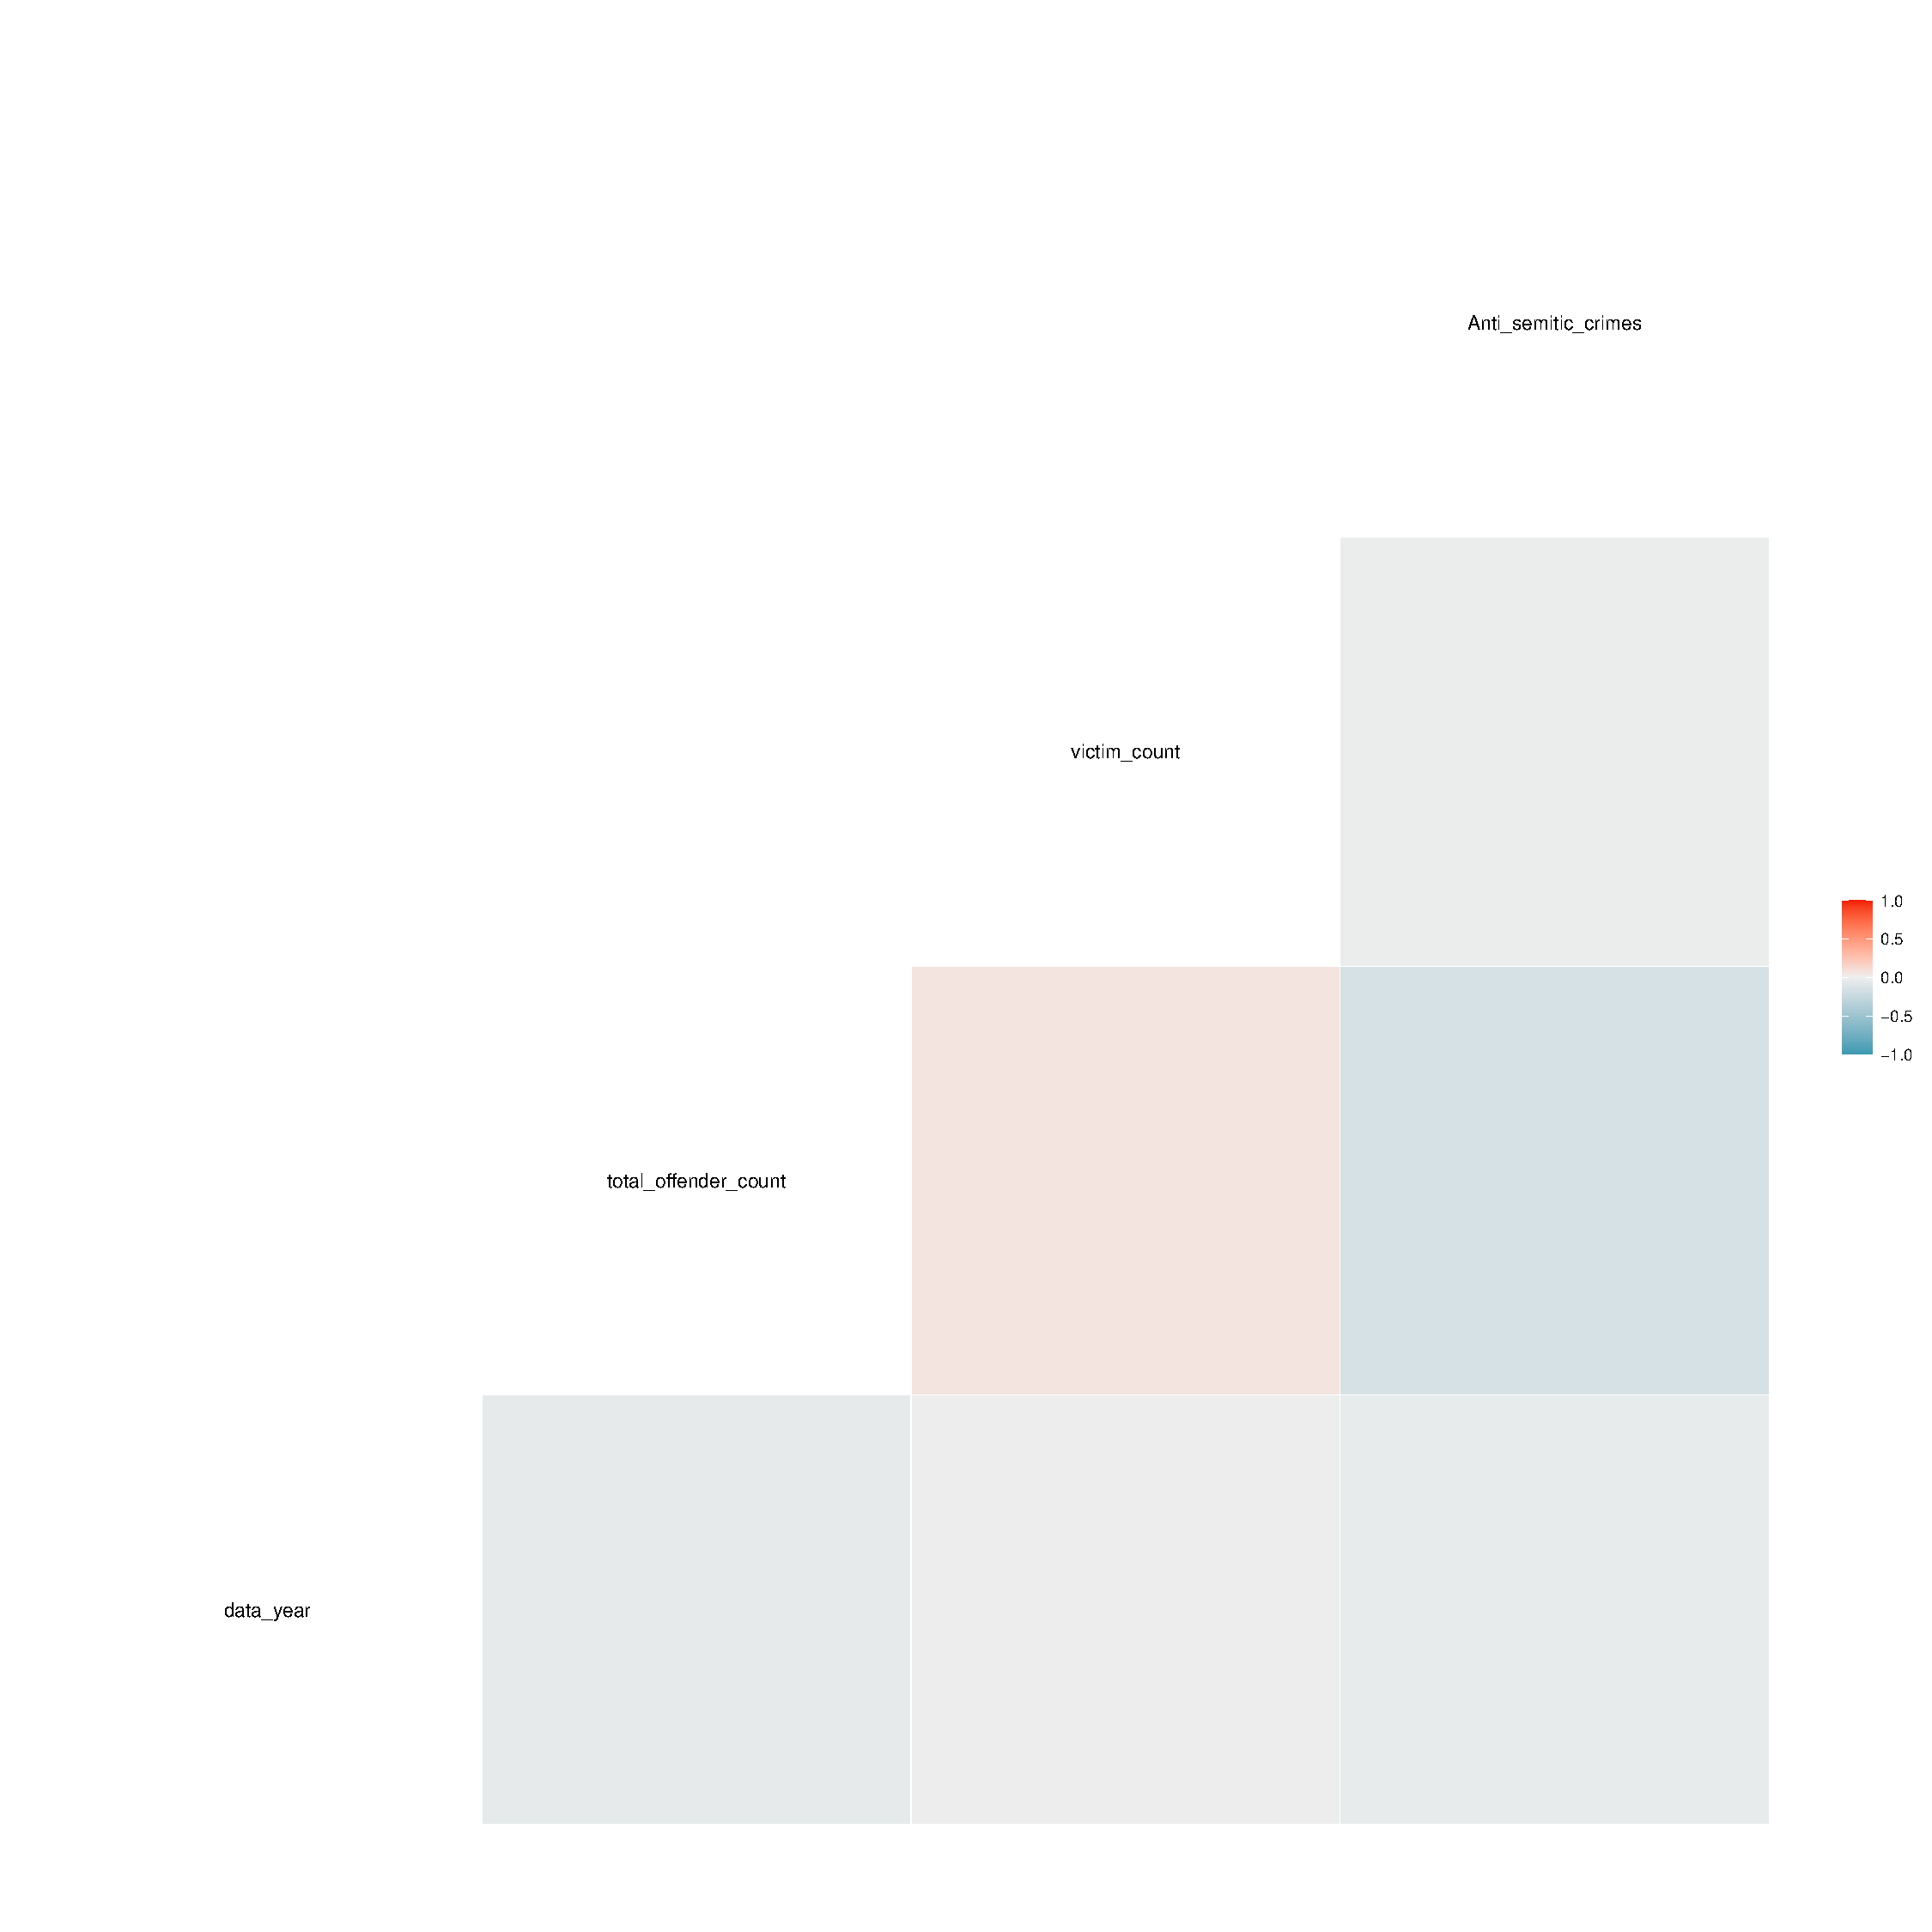
\includegraphics{Data_621_HW_5_files/figure-latex/unnamed-chunk-12-1.pdf}

\hypertarget{df_wine_train}{%
\subsubsection{df\_wine\_train}\label{df_wine_train}}

\hypertarget{summary-statistics-1}{%
\paragraph{Summary Statistics}\label{summary-statistics-1}}

\begin{Shaded}
\begin{Highlighting}[]
\FunctionTok{describe}\NormalTok{(df\_wine\_train)}
\end{Highlighting}
\end{Shaded}

\begin{verbatim}
##                    vars     n    mean      sd  median trimmed     mad     min
## INDEX                 1 12795 8069.98 4656.91 8110.00 8071.03 5977.84    1.00
## TARGET                2 12795    3.03    1.93    3.00    3.05    1.48    0.00
## FixedAcidity          3 12795    7.08    6.32    6.90    7.07    3.26  -18.10
## VolatileAcidity       4 12795    0.32    0.78    0.28    0.32    0.43   -2.79
## CitricAcid            5 12795    0.31    0.86    0.31    0.31    0.42   -3.24
## ResidualSugar         6 12179    5.42   33.75    3.90    5.58   15.72 -127.80
## Chlorides             7 12157    0.05    0.32    0.05    0.05    0.13   -1.17
## FreeSulfurDioxide     8 12148   30.85  148.71   30.00   30.93   56.34 -555.00
## TotalSulfurDioxide    9 12113  120.71  231.91  123.00  120.89  134.92 -823.00
## Density              10 12795    0.99    0.03    0.99    0.99    0.01    0.89
## pH                   11 12400    3.21    0.68    3.20    3.21    0.39    0.48
## Sulphates            12 11585    0.53    0.93    0.50    0.53    0.44   -3.13
## Alcohol              13 12142   10.49    3.73   10.40   10.50    2.37   -4.70
## LabelAppeal          14 12795   -0.01    0.89    0.00   -0.01    1.48   -2.00
## AcidIndex            15 12795    7.77    1.32    8.00    7.64    1.48    4.00
## STARS                16  9436    2.04    0.90    2.00    1.97    1.48    1.00
##                         max    range  skew kurtosis    se
## INDEX              16129.00 16128.00  0.00    -1.20 41.17
## TARGET                 8.00     8.00 -0.33    -0.88  0.02
## FixedAcidity          34.40    52.50 -0.02     1.67  0.06
## VolatileAcidity        3.68     6.47  0.02     1.83  0.01
## CitricAcid             3.86     7.10 -0.05     1.84  0.01
## ResidualSugar        141.15   268.95 -0.05     1.88  0.31
## Chlorides              1.35     2.52  0.03     1.79  0.00
## FreeSulfurDioxide    623.00  1178.00  0.01     1.84  1.35
## TotalSulfurDioxide  1057.00  1880.00 -0.01     1.67  2.11
## Density                1.10     0.21 -0.02     1.90  0.00
## pH                     6.13     5.65  0.04     1.65  0.01
## Sulphates              4.24     7.37  0.01     1.75  0.01
## Alcohol               26.50    31.20 -0.03     1.54  0.03
## LabelAppeal            2.00     4.00  0.01    -0.26  0.01
## AcidIndex             17.00    13.00  1.65     5.19  0.01
## STARS                  4.00     3.00  0.45    -0.69  0.01
\end{verbatim}

\begin{Shaded}
\begin{Highlighting}[]
\FunctionTok{summary}\NormalTok{(df\_wine\_train)}
\end{Highlighting}
\end{Shaded}

\begin{verbatim}
##      INDEX           TARGET       FixedAcidity     VolatileAcidity  
##  Min.   :    1   Min.   :0.000   Min.   :-18.100   Min.   :-2.7900  
##  1st Qu.: 4038   1st Qu.:2.000   1st Qu.:  5.200   1st Qu.: 0.1300  
##  Median : 8110   Median :3.000   Median :  6.900   Median : 0.2800  
##  Mean   : 8070   Mean   :3.029   Mean   :  7.076   Mean   : 0.3241  
##  3rd Qu.:12106   3rd Qu.:4.000   3rd Qu.:  9.500   3rd Qu.: 0.6400  
##  Max.   :16129   Max.   :8.000   Max.   : 34.400   Max.   : 3.6800  
##                                                                     
##    CitricAcid      ResidualSugar        Chlorides       FreeSulfurDioxide
##  Min.   :-3.2400   Min.   :-127.800   Min.   :-1.1710   Min.   :-555.00  
##  1st Qu.: 0.0300   1st Qu.:  -2.000   1st Qu.:-0.0310   1st Qu.:   0.00  
##  Median : 0.3100   Median :   3.900   Median : 0.0460   Median :  30.00  
##  Mean   : 0.3084   Mean   :   5.419   Mean   : 0.0548   Mean   :  30.85  
##  3rd Qu.: 0.5800   3rd Qu.:  15.900   3rd Qu.: 0.1530   3rd Qu.:  70.00  
##  Max.   : 3.8600   Max.   : 141.150   Max.   : 1.3510   Max.   : 623.00  
##                    NA's   :616        NA's   :638       NA's   :647      
##  TotalSulfurDioxide    Density             pH          Sulphates      
##  Min.   :-823.0     Min.   :0.8881   Min.   :0.480   Min.   :-3.1300  
##  1st Qu.:  27.0     1st Qu.:0.9877   1st Qu.:2.960   1st Qu.: 0.2800  
##  Median : 123.0     Median :0.9945   Median :3.200   Median : 0.5000  
##  Mean   : 120.7     Mean   :0.9942   Mean   :3.208   Mean   : 0.5271  
##  3rd Qu.: 208.0     3rd Qu.:1.0005   3rd Qu.:3.470   3rd Qu.: 0.8600  
##  Max.   :1057.0     Max.   :1.0992   Max.   :6.130   Max.   : 4.2400  
##  NA's   :682                         NA's   :395     NA's   :1210     
##     Alcohol       LabelAppeal          AcidIndex          STARS      
##  Min.   :-4.70   Min.   :-2.000000   Min.   : 4.000   Min.   :1.000  
##  1st Qu.: 9.00   1st Qu.:-1.000000   1st Qu.: 7.000   1st Qu.:1.000  
##  Median :10.40   Median : 0.000000   Median : 8.000   Median :2.000  
##  Mean   :10.49   Mean   :-0.009066   Mean   : 7.773   Mean   :2.042  
##  3rd Qu.:12.40   3rd Qu.: 1.000000   3rd Qu.: 8.000   3rd Qu.:3.000  
##  Max.   :26.50   Max.   : 2.000000   Max.   :17.000   Max.   :4.000  
##  NA's   :653                                          NA's   :3359
\end{verbatim}

\begin{Shaded}
\begin{Highlighting}[]
\FunctionTok{str}\NormalTok{(df\_wine\_train)}
\end{Highlighting}
\end{Shaded}

\begin{verbatim}
## 'data.frame':    12795 obs. of  16 variables:
##  $ INDEX             : int  1 2 4 5 6 7 8 11 12 13 ...
##  $ TARGET            : int  3 3 5 3 4 0 0 4 3 6 ...
##  $ FixedAcidity      : num  3.2 4.5 7.1 5.7 8 11.3 7.7 6.5 14.8 5.5 ...
##  $ VolatileAcidity   : num  1.16 0.16 2.64 0.385 0.33 0.32 0.29 -1.22 0.27 -0.22 ...
##  $ CitricAcid        : num  -0.98 -0.81 -0.88 0.04 -1.26 0.59 -0.4 0.34 1.05 0.39 ...
##  $ ResidualSugar     : num  54.2 26.1 14.8 18.8 9.4 ...
##  $ Chlorides         : num  -0.567 -0.425 0.037 -0.425 NA 0.556 0.06 0.04 -0.007 -0.277 ...
##  $ FreeSulfurDioxide : num  NA 15 214 22 -167 -37 287 523 -213 62 ...
##  $ TotalSulfurDioxide: num  268 -327 142 115 108 15 156 551 NA 180 ...
##  $ Density           : num  0.993 1.028 0.995 0.996 0.995 ...
##  $ pH                : num  3.33 3.38 3.12 2.24 3.12 3.2 3.49 3.2 4.93 3.09 ...
##  $ Sulphates         : num  -0.59 0.7 0.48 1.83 1.77 1.29 1.21 NA 0.26 0.75 ...
##  $ Alcohol           : num  9.9 NA 22 6.2 13.7 15.4 10.3 11.6 15 12.6 ...
##  $ LabelAppeal       : int  0 -1 -1 -1 0 0 0 1 0 0 ...
##  $ AcidIndex         : int  8 7 8 6 9 11 8 7 6 8 ...
##  $ STARS             : int  2 3 3 1 2 NA NA 3 NA 4 ...
\end{verbatim}

\hypertarget{missing-data-1}{%
\paragraph{Missing Data}\label{missing-data-1}}

\begin{Shaded}
\begin{Highlighting}[]
\ControlFlowTok{for}\NormalTok{ (i }\ControlFlowTok{in} \FunctionTok{colnames}\NormalTok{(df\_wine\_train))\{}
  \FunctionTok{print}\NormalTok{(}\FunctionTok{paste}\NormalTok{(i,}\StringTok{"  "}\NormalTok{, }\FunctionTok{sum}\NormalTok{(}\FunctionTok{is.na}\NormalTok{(df\_wine\_train[,i])),}\AttributeTok{sep =} \StringTok{""}\NormalTok{))}
\NormalTok{\}}
\end{Highlighting}
\end{Shaded}

\begin{verbatim}
## [1] "INDEX  0"
## [1] "TARGET  0"
## [1] "FixedAcidity  0"
## [1] "VolatileAcidity  0"
## [1] "CitricAcid  0"
## [1] "ResidualSugar  616"
## [1] "Chlorides  638"
## [1] "FreeSulfurDioxide  647"
## [1] "TotalSulfurDioxide  682"
## [1] "Density  0"
## [1] "pH  395"
## [1] "Sulphates  1210"
## [1] "Alcohol  653"
## [1] "LabelAppeal  0"
## [1] "AcidIndex  0"
## [1] "STARS  3359"
\end{verbatim}

\hypertarget{outliers-1}{%
\paragraph{Outliers}\label{outliers-1}}

\begin{Shaded}
\begin{Highlighting}[]
\NormalTok{df\_wine\_train }\SpecialCharTok{\%\textgreater{}\%}
  \FunctionTok{scale}\NormalTok{() }\SpecialCharTok{\%\textgreater{}\%}
  \FunctionTok{as.data.frame}\NormalTok{() }\SpecialCharTok{\%\textgreater{}\%}
  \FunctionTok{stack}\NormalTok{() }\SpecialCharTok{\%\textgreater{}\%}
  \FunctionTok{ggplot}\NormalTok{(}\FunctionTok{aes}\NormalTok{(}\AttributeTok{x =}\NormalTok{ ind, }\AttributeTok{y =}\NormalTok{ values)) }\SpecialCharTok{+}
  \FunctionTok{geom\_boxplot}\NormalTok{() }\SpecialCharTok{+}
  \FunctionTok{labs}\NormalTok{(}\AttributeTok{title =} \StringTok{\textquotesingle{}Boxplot Training (scaled)\textquotesingle{}}\NormalTok{,}
       \AttributeTok{x =} \StringTok{\textquotesingle{}Variables\textquotesingle{}}\NormalTok{,}
       \AttributeTok{y =} \StringTok{\textquotesingle{}Normalized\_Values\textquotesingle{}}\NormalTok{)}\SpecialCharTok{+}
  \FunctionTok{theme}\NormalTok{(}\AttributeTok{axis.text.x=}\FunctionTok{element\_text}\NormalTok{(}\AttributeTok{size=}\DecValTok{10}\NormalTok{, }\AttributeTok{angle=}\DecValTok{90}\NormalTok{)) }
\end{Highlighting}
\end{Shaded}

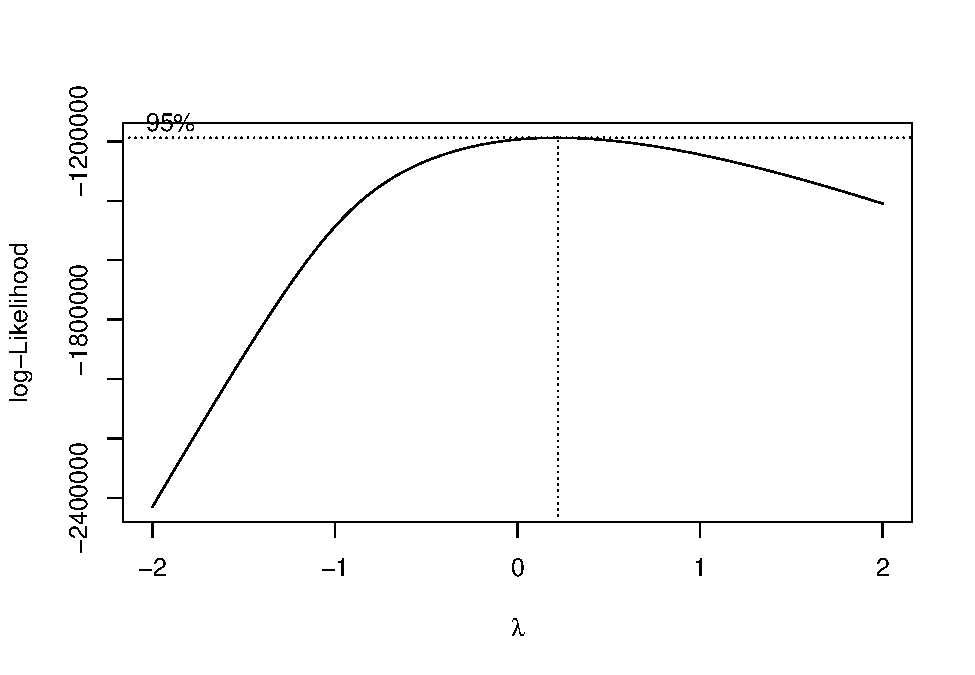
\includegraphics{Data_621_HW_5_files/figure-latex/unnamed-chunk-18-1.pdf}

(Melissa's added part)

\hypertarget{data-exploration}{%
\section{DATA EXPLORATION}\label{data-exploration}}

\begin{Shaded}
\begin{Highlighting}[]
\FunctionTok{print}\NormalTok{(}\FunctionTok{skim}\NormalTok{(df\_wine\_train))}
\end{Highlighting}
\end{Shaded}

\begin{verbatim}
## -- Data Summary ------------------------
##                            Values       
## Name                       df_wine_train
## Number of rows             12795        
## Number of columns          16           
## _______________________                 
## Column type frequency:                  
##   numeric                  16           
## ________________________                
## Group variables            None         
## 
## -- Variable type: numeric ------------------------------------------------------
##    skim_variable      n_missing complete_rate       mean        sd       p0
##  1 INDEX                      0         1     8070.      4657.        1    
##  2 TARGET                     0         1        3.03       1.93      0    
##  3 FixedAcidity               0         1        7.08       6.32    -18.1  
##  4 VolatileAcidity            0         1        0.324      0.784    -2.79 
##  5 CitricAcid                 0         1        0.308      0.862    -3.24 
##  6 ResidualSugar            616         0.952    5.42      33.7    -128.   
##  7 Chlorides                638         0.950    0.0548     0.318    -1.17 
##  8 FreeSulfurDioxide        647         0.949   30.8      149.     -555    
##  9 TotalSulfurDioxide       682         0.947  121.       232.     -823    
## 10 Density                    0         1        0.994      0.0265    0.888
## 11 pH                       395         0.969    3.21       0.680     0.48 
## 12 Sulphates               1210         0.905    0.527      0.932    -3.13 
## 13 Alcohol                  653         0.949   10.5        3.73     -4.7  
## 14 LabelAppeal                0         1       -0.00907    0.891    -2    
## 15 AcidIndex                  0         1        7.77       1.32      4    
## 16 STARS                   3359         0.737    2.04       0.903     1    
##         p25      p50       p75     p100 hist 
##  1 4038.    8110     12106.    16129    ▇▇▇▇▇
##  2    2        3         4         8    ▆▇▇▆▁
##  3    5.2      6.9       9.5      34.4  ▁▂▇▂▁
##  4    0.13     0.28      0.64      3.68 ▁▂▇▂▁
##  5    0.03     0.31      0.58      3.86 ▁▂▇▂▁
##  6   -2        3.9      15.9     141.   ▁▂▇▂▁
##  7   -0.031    0.046     0.153     1.35 ▁▂▇▂▁
##  8    0       30        70       623    ▁▂▇▂▁
##  9   27      123       208      1057    ▁▂▇▂▁
## 10    0.988    0.994     1.00      1.10 ▁▂▇▂▁
## 11    2.96     3.2       3.47      6.13 ▁▂▇▂▁
## 12    0.28     0.5       0.86      4.24 ▁▂▇▂▁
## 13    9       10.4      12.4      26.5  ▁▂▇▂▁
## 14   -1        0         1         2    ▁▅▇▅▁
## 15    7        8         8        17    ▁▇▁▁▁
## 16    1        2         3         4    ▇▇▁▅▂
\end{verbatim}

\begin{Shaded}
\begin{Highlighting}[]
\FunctionTok{summary}\NormalTok{(df\_wine\_train)}
\end{Highlighting}
\end{Shaded}

\begin{verbatim}
##      INDEX           TARGET       FixedAcidity     VolatileAcidity  
##  Min.   :    1   Min.   :0.000   Min.   :-18.100   Min.   :-2.7900  
##  1st Qu.: 4038   1st Qu.:2.000   1st Qu.:  5.200   1st Qu.: 0.1300  
##  Median : 8110   Median :3.000   Median :  6.900   Median : 0.2800  
##  Mean   : 8070   Mean   :3.029   Mean   :  7.076   Mean   : 0.3241  
##  3rd Qu.:12106   3rd Qu.:4.000   3rd Qu.:  9.500   3rd Qu.: 0.6400  
##  Max.   :16129   Max.   :8.000   Max.   : 34.400   Max.   : 3.6800  
##                                                                     
##    CitricAcid      ResidualSugar        Chlorides       FreeSulfurDioxide
##  Min.   :-3.2400   Min.   :-127.800   Min.   :-1.1710   Min.   :-555.00  
##  1st Qu.: 0.0300   1st Qu.:  -2.000   1st Qu.:-0.0310   1st Qu.:   0.00  
##  Median : 0.3100   Median :   3.900   Median : 0.0460   Median :  30.00  
##  Mean   : 0.3084   Mean   :   5.419   Mean   : 0.0548   Mean   :  30.85  
##  3rd Qu.: 0.5800   3rd Qu.:  15.900   3rd Qu.: 0.1530   3rd Qu.:  70.00  
##  Max.   : 3.8600   Max.   : 141.150   Max.   : 1.3510   Max.   : 623.00  
##                    NA's   :616        NA's   :638       NA's   :647      
##  TotalSulfurDioxide    Density             pH          Sulphates      
##  Min.   :-823.0     Min.   :0.8881   Min.   :0.480   Min.   :-3.1300  
##  1st Qu.:  27.0     1st Qu.:0.9877   1st Qu.:2.960   1st Qu.: 0.2800  
##  Median : 123.0     Median :0.9945   Median :3.200   Median : 0.5000  
##  Mean   : 120.7     Mean   :0.9942   Mean   :3.208   Mean   : 0.5271  
##  3rd Qu.: 208.0     3rd Qu.:1.0005   3rd Qu.:3.470   3rd Qu.: 0.8600  
##  Max.   :1057.0     Max.   :1.0992   Max.   :6.130   Max.   : 4.2400  
##  NA's   :682                         NA's   :395     NA's   :1210     
##     Alcohol       LabelAppeal          AcidIndex          STARS      
##  Min.   :-4.70   Min.   :-2.000000   Min.   : 4.000   Min.   :1.000  
##  1st Qu.: 9.00   1st Qu.:-1.000000   1st Qu.: 7.000   1st Qu.:1.000  
##  Median :10.40   Median : 0.000000   Median : 8.000   Median :2.000  
##  Mean   :10.49   Mean   :-0.009066   Mean   : 7.773   Mean   :2.042  
##  3rd Qu.:12.40   3rd Qu.: 1.000000   3rd Qu.: 8.000   3rd Qu.:3.000  
##  Max.   :26.50   Max.   : 2.000000   Max.   :17.000   Max.   :4.000  
##  NA's   :653                                          NA's   :3359
\end{verbatim}

Of evaluated variable:

\begin{Shaded}
\begin{Highlighting}[]
\FunctionTok{print}\NormalTok{(}\FunctionTok{skim}\NormalTok{(df\_wine\_eval))}
\end{Highlighting}
\end{Shaded}

\begin{verbatim}
## -- Data Summary ------------------------
##                            Values      
## Name                       df_wine_eval
## Number of rows             3335        
## Number of columns          16          
## _______________________                
## Column type frequency:                 
##   logical                  1           
##   numeric                  15          
## ________________________               
## Group variables            None        
## 
## -- Variable type: logical ------------------------------------------------------
##   skim_variable n_missing complete_rate mean count
## 1 TARGET             3335             0  NaN ": " 
## 
## -- Variable type: numeric ------------------------------------------------------
##    skim_variable      n_missing complete_rate      mean        sd       p0
##  1 IN                         0         1     8048.     4655.        3    
##  2 FixedAcidity               0         1        6.86      6.32    -18.2  
##  3 VolatileAcidity            0         1        0.310     0.807    -2.83 
##  4 CitricAcid                 0         1        0.312     0.871    -3.12 
##  5 ResidualSugar            168         0.950    5.32     34.4    -128.   
##  6 Chlorides                138         0.959    0.0614    0.314    -1.15 
##  7 FreeSulfurDioxide        152         0.954   34.9     150.     -563    
##  8 TotalSulfurDioxide       157         0.953  123.      226.     -769    
##  9 Density                    0         1        0.995     0.0262    0.890
## 10 pH                       104         0.969    3.24      0.676     0.6  
## 11 Sulphates                310         0.907    0.535     0.905    -3.07 
## 12 Alcohol                  185         0.945   10.6       3.76     -4.2  
## 13 LabelAppeal                0         1        0.0135    0.889    -2    
## 14 AcidIndex                  0         1        7.75      1.32      5    
## 15 STARS                    841         0.748    2.04      0.913     1    
##         p25      p50       p75     p100 hist 
##  1 4018.    7906     12061     16130    ▇▇▇▇▇
##  2    5.2      6.9       9        33.5  ▁▂▇▂▁
##  3    0.08     0.28      0.63      3.61 ▁▂▇▂▁
##  4    0        0.31      0.605     3.76 ▁▂▇▂▁
##  5   -2.6      3.6      17.2     145.   ▁▂▇▂▁
##  6    0.016    0.047     0.171     1.26 ▁▂▇▂▁
##  7    3       30        79.2     617    ▁▂▇▂▁
##  8   27.2    124       210      1004    ▁▂▇▂▁
##  9    0.988    0.995     1.00      1.10 ▁▂▇▂▁
## 10    2.98     3.21      3.49      6.21 ▁▂▇▂▁
## 11    0.33     0.5       0.82      4.18 ▁▂▇▂▁
## 12    9       10.4      12.5      25.6  ▁▂▇▂▁
## 13   -1        0         1         2    ▁▅▇▅▁
## 14    7        8         8        17    ▇▇▁▁▁
## 15    1        2         3         4    ▇▇▁▅▂
\end{verbatim}

\begin{Shaded}
\begin{Highlighting}[]
\FunctionTok{summary}\NormalTok{(df\_wine\_eval)}
\end{Highlighting}
\end{Shaded}

\begin{verbatim}
##        IN         TARGET         FixedAcidity     VolatileAcidity  
##  Min.   :    3   Mode:logical   Min.   :-18.200   Min.   :-2.8300  
##  1st Qu.: 4018   NA's:3335      1st Qu.:  5.200   1st Qu.: 0.0800  
##  Median : 7906                  Median :  6.900   Median : 0.2800  
##  Mean   : 8048                  Mean   :  6.864   Mean   : 0.3103  
##  3rd Qu.:12061                  3rd Qu.:  9.000   3rd Qu.: 0.6300  
##  Max.   :16130                  Max.   : 33.500   Max.   : 3.6100  
##                                                                    
##    CitricAcid      ResidualSugar        Chlorides        FreeSulfurDioxide
##  Min.   :-3.1200   Min.   :-128.300   Min.   :-1.15000   Min.   :-563.00  
##  1st Qu.: 0.0000   1st Qu.:  -2.600   1st Qu.: 0.01600   1st Qu.:   3.00  
##  Median : 0.3100   Median :   3.600   Median : 0.04700   Median :  30.00  
##  Mean   : 0.3124   Mean   :   5.319   Mean   : 0.06143   Mean   :  34.95  
##  3rd Qu.: 0.6050   3rd Qu.:  17.200   3rd Qu.: 0.17100   3rd Qu.:  79.25  
##  Max.   : 3.7600   Max.   : 145.400   Max.   : 1.26300   Max.   : 617.00  
##                    NA's   :168        NA's   :138        NA's   :152      
##  TotalSulfurDioxide    Density             pH          Sulphates      
##  Min.   :-769.00    Min.   :0.8898   Min.   :0.600   Min.   :-3.0700  
##  1st Qu.:  27.25    1st Qu.:0.9883   1st Qu.:2.980   1st Qu.: 0.3300  
##  Median : 124.00    Median :0.9946   Median :3.210   Median : 0.5000  
##  Mean   : 123.41    Mean   :0.9947   Mean   :3.237   Mean   : 0.5346  
##  3rd Qu.: 210.00    3rd Qu.:1.0005   3rd Qu.:3.490   3rd Qu.: 0.8200  
##  Max.   :1004.00    Max.   :1.0998   Max.   :6.210   Max.   : 4.1800  
##  NA's   :157                         NA's   :104     NA's   :310      
##     Alcohol       LabelAppeal         AcidIndex          STARS     
##  Min.   :-4.20   Min.   :-2.00000   Min.   : 5.000   Min.   :1.00  
##  1st Qu.: 9.00   1st Qu.:-1.00000   1st Qu.: 7.000   1st Qu.:1.00  
##  Median :10.40   Median : 0.00000   Median : 8.000   Median :2.00  
##  Mean   :10.58   Mean   : 0.01349   Mean   : 7.748   Mean   :2.04  
##  3rd Qu.:12.50   3rd Qu.: 1.00000   3rd Qu.: 8.000   3rd Qu.:3.00  
##  Max.   :25.60   Max.   : 2.00000   Max.   :17.000   Max.   :4.00  
##  NA's   :185                                         NA's   :841
\end{verbatim}

Looking at histogram

\begin{Shaded}
\begin{Highlighting}[]
\CommentTok{\# Gather the data into a long format}
\NormalTok{data\_long }\OtherTok{\textless{}{-}} \FunctionTok{gather}\NormalTok{(df\_wine\_train, }\AttributeTok{key =} \StringTok{"Variable"}\NormalTok{, }\AttributeTok{value =} \StringTok{"Value"}\NormalTok{)}

\FunctionTok{ggplot}\NormalTok{(data\_long, }\FunctionTok{aes}\NormalTok{(}\AttributeTok{x =}\NormalTok{ Value)) }\SpecialCharTok{+}
  \FunctionTok{geom\_histogram}\NormalTok{() }\SpecialCharTok{+}
  \FunctionTok{facet\_wrap}\NormalTok{(}\SpecialCharTok{\textasciitilde{}}\NormalTok{Variable, }\AttributeTok{scales =} \StringTok{"free"}\NormalTok{) }\SpecialCharTok{+}
  \FunctionTok{labs}\NormalTok{(}\AttributeTok{title =} \StringTok{"Histogram of Variables"}\NormalTok{)}
\end{Highlighting}
\end{Shaded}

\begin{verbatim}
## `stat_bin()` using `bins = 30`. Pick better value with `binwidth`.
\end{verbatim}

\begin{verbatim}
## Warning: Removed 8200 rows containing non-finite values (`stat_bin()`).
\end{verbatim}

\includegraphics{Data_621_HW_5_files/figure-latex/unnamed-chunk-24-1.pdf}

Relatively normal data. We do not have to correct any variables

\begin{Shaded}
\begin{Highlighting}[]
\CommentTok{\# Create a correlation matrix for all variables}
\NormalTok{(cor\_matrix }\OtherTok{\textless{}{-}} \FunctionTok{cor}\NormalTok{(df\_wine\_train, }\AttributeTok{use=}\StringTok{\textquotesingle{}complete.obs\textquotesingle{}}\NormalTok{))}
\end{Highlighting}
\end{Shaded}

\begin{verbatim}
##                            INDEX        TARGET FixedAcidity VolatileAcidity
## INDEX               1.0000000000  0.0236764338 -0.002831415   -0.0008743296
## TARGET              0.0236764338  1.0000000000 -0.012538100   -0.0759978765
## FixedAcidity       -0.0028314152 -0.0125380998  1.000000000    0.0190109733
## VolatileAcidity    -0.0008743296 -0.0759978765  0.019010973    1.0000000000
## CitricAcid          0.0278869710  0.0023450490  0.014000376   -0.0234315631
## ResidualSugar       0.0208952098  0.0035195999 -0.015429391    0.0015279517
## Chlorides           0.0026827829 -0.0304301331 -0.006104447    0.0148489225
## FreeSulfurDioxide   0.0046416504  0.0226398054  0.015438463   -0.0114408079
## TotalSulfurDioxide  0.0064949038  0.0216020726 -0.023323485   -0.0007434083
## Density            -0.0034840089 -0.0475989086  0.011574241    0.0130977690
## pH                 -0.0274556333  0.0002198557 -0.004553886    0.0072030364
## Sulphates          -0.0053946247 -0.0212203783  0.042229181    0.0015161001
## Alcohol            -0.0024453460  0.0737771084 -0.013085026    0.0002603082
## LabelAppeal         0.0314911460  0.4979464796  0.011375965   -0.0202419713
## AcidIndex           0.0055244862 -0.1676430648  0.154167846    0.0250529742
## STARS              -0.0057807296  0.5546857223 -0.004937345   -0.0402432388
##                       CitricAcid ResidualSugar     Chlorides FreeSulfurDioxide
## INDEX               0.0278869710   0.020895210  0.0026827829       0.004641650
## TARGET              0.0023450490   0.003519600 -0.0304301331       0.022639805
## FixedAcidity        0.0140003760  -0.015429391 -0.0061044471       0.015438463
## VolatileAcidity    -0.0234315631   0.001527952  0.0148489225      -0.011440808
## CitricAcid          1.0000000000  -0.009843146 -0.0335608661       0.012113248
## ResidualSugar      -0.0098431456   1.000000000  0.0041215692       0.021959113
## Chlorides          -0.0335608661   0.004121569  1.0000000000      -0.020492488
## FreeSulfurDioxide   0.0121132485   0.021959113 -0.0204924876       1.000000000
## TotalSulfurDioxide -0.0099174506   0.017030939  0.0004188605       0.013461673
## Density            -0.0169919691  -0.007120841  0.0206724860      -0.008663509
## pH                 -0.0007581304   0.017563769 -0.0179702278      -0.002008516
## Sulphates          -0.0144237270  -0.002705775  0.0026187777       0.026829029
## Alcohol             0.0169864284  -0.018943324 -0.0228849573      -0.023867458
## LabelAppeal         0.0153315666  -0.004579308 -0.0063870237       0.014960087
## AcidIndex           0.0545838104  -0.020301890 -0.0017134096      -0.014733717
## STARS               0.0071401699   0.019665541 -0.0063242568      -0.015390398
##                    TotalSulfurDioxide      Density            pH    Sulphates
## INDEX                    0.0064949038 -0.003484009 -0.0274556333 -0.005394625
## TARGET                   0.0216020726 -0.047598909  0.0002198557 -0.021220378
## FixedAcidity            -0.0233234848  0.011574241 -0.0045538857  0.042229181
## VolatileAcidity         -0.0007434083  0.013097769  0.0072030364  0.001516100
## CitricAcid              -0.0099174506 -0.016991969 -0.0007581304 -0.014423727
## ResidualSugar            0.0170309394 -0.007120841  0.0175637691 -0.002705775
## Chlorides                0.0004188605  0.020672486 -0.0179702278  0.002618778
## FreeSulfurDioxide        0.0134616726 -0.008663509 -0.0020085157  0.026829029
## TotalSulfurDioxide       1.0000000000  0.023167955 -0.0034227601  0.002504051
## Density                  0.0231679548  1.000000000 -0.0020192285 -0.010609294
## pH                      -0.0034227601 -0.002019229  1.0000000000  0.010449255
## Sulphates                0.0025040509 -0.010609294  0.0104492547  1.000000000
## Alcohol                 -0.0168515467 -0.006128355 -0.0122034469  0.010844330
## LabelAppeal             -0.0027237419 -0.018094403  0.0002181758  0.003768700
## AcidIndex               -0.0221292631  0.047778830 -0.0537128921  0.031071782
## STARS                    0.0220949002 -0.028492455 -0.0044002985 -0.023135130
##                          Alcohol   LabelAppeal    AcidIndex        STARS
## INDEX              -0.0024453460  0.0314911460  0.005524486 -0.005780730
## TARGET              0.0737771084  0.4979464796 -0.167643065  0.554685722
## FixedAcidity       -0.0130850260  0.0113759650  0.154167846 -0.004937345
## VolatileAcidity     0.0002603082 -0.0202419713  0.025052974 -0.040243239
## CitricAcid          0.0169864284  0.0153315666  0.054583810  0.007140170
## ResidualSugar      -0.0189433242 -0.0045793083 -0.020301890  0.019665541
## Chlorides          -0.0228849573 -0.0063870237 -0.001713410 -0.006324257
## FreeSulfurDioxide  -0.0238674577  0.0149600871 -0.014733717 -0.015390398
## TotalSulfurDioxide -0.0168515467 -0.0027237419 -0.022129263  0.022094900
## Density            -0.0061283546 -0.0180944026  0.047778830 -0.028492455
## pH                 -0.0122034469  0.0002181758 -0.053712892 -0.004400299
## Sulphates           0.0108443299  0.0037686996  0.031071782 -0.023135130
## Alcohol             1.0000000000 -0.0006449123 -0.055891906  0.064854486
## LabelAppeal        -0.0006449123  1.0000000000  0.010300984  0.318897022
## AcidIndex          -0.0558919056  0.0103009840  1.000000000 -0.095482582
## STARS               0.0648544864  0.3188970216 -0.095482582  1.000000000
\end{verbatim}

Only 3 real variable that relate to TARGET which are LabelAppeal,
AcidIndex, STARS. STARS though has a lot of NA values

\begin{Shaded}
\begin{Highlighting}[]
\CommentTok{\# Plot a histogram}
\FunctionTok{hist}\NormalTok{(df\_wine\_train}\SpecialCharTok{$}\NormalTok{TARGET, }\AttributeTok{main =} \StringTok{"Histogram of TARGET"}\NormalTok{, }\AttributeTok{xlab =} \StringTok{"TARGET"}\NormalTok{, }\AttributeTok{col =} \StringTok{"skyblue"}\NormalTok{, }\AttributeTok{border =} \StringTok{"black"}\NormalTok{)}
\end{Highlighting}
\end{Shaded}

\includegraphics{Data_621_HW_5_files/figure-latex/unnamed-chunk-26-1.pdf}

\begin{Shaded}
\begin{Highlighting}[]
\CommentTok{\# Calculate the percentage of unique values in the TARGET variable}
\NormalTok{target\_table }\OtherTok{\textless{}{-}} \FunctionTok{table}\NormalTok{(df\_wine\_train}\SpecialCharTok{$}\NormalTok{TARGET)}
\NormalTok{target\_percentage }\OtherTok{\textless{}{-}} \FunctionTok{prop.table}\NormalTok{(target\_table) }\SpecialCharTok{*} \DecValTok{100}


\NormalTok{rounded\_percentage }\OtherTok{\textless{}{-}} \FunctionTok{round}\NormalTok{(target\_percentage, }\DecValTok{2}\NormalTok{)}


\FunctionTok{print}\NormalTok{(rounded\_percentage)}
\end{Highlighting}
\end{Shaded}

\begin{verbatim}
## 
##     0     1     2     3     4     5     6     7     8 
## 21.37  1.91  8.53 20.41 24.83 15.74  5.98  1.11  0.13
\end{verbatim}

\begin{Shaded}
\begin{Highlighting}[]
\NormalTok{df\_wine\_train }\SpecialCharTok{\%\textgreater{}\%} 
  \FunctionTok{mutate}\NormalTok{(}\AttributeTok{STARS =} \FunctionTok{as.factor}\NormalTok{(STARS),}
         \AttributeTok{TARGET =} \FunctionTok{as.factor}\NormalTok{(TARGET)) }\SpecialCharTok{\%\textgreater{}\%} 
  \FunctionTok{ggplot}\NormalTok{(}\FunctionTok{aes}\NormalTok{(STARS)) }\SpecialCharTok{+}
  \FunctionTok{geom\_bar}\NormalTok{(}\FunctionTok{aes}\NormalTok{(}\AttributeTok{fill =}\NormalTok{ TARGET)) }\SpecialCharTok{+}
  \FunctionTok{scale\_fill\_brewer}\NormalTok{(}\AttributeTok{palette =} \StringTok{"RdYlGn"}\NormalTok{) }
\end{Highlighting}
\end{Shaded}

\includegraphics{Data_621_HW_5_files/figure-latex/unnamed-chunk-28-1.pdf}

Because STARS has a lot of NA values that relate to a TARGET value of 0
we should make STARS NA zero instead of eliminating NA values.

\hypertarget{data-preparation}{%
\section{DATA PREPARATION}\label{data-preparation}}

\begin{Shaded}
\begin{Highlighting}[]
\NormalTok{df\_wine\_train\_transformed }\OtherTok{\textless{}{-}}\NormalTok{ df\_wine\_train }\SpecialCharTok{\%\textgreater{}\%} 
    \FunctionTok{mutate}\NormalTok{(}\AttributeTok{STARS =} \FunctionTok{replace}\NormalTok{(STARS, }\FunctionTok{is.na}\NormalTok{(STARS) , }\DecValTok{0}\NormalTok{))}

\NormalTok{df\_wine\_eval\_transformed  }\OtherTok{\textless{}{-}}\NormalTok{ df\_wine\_eval }\SpecialCharTok{\%\textgreater{}\%} 
    \FunctionTok{mutate}\NormalTok{(}\AttributeTok{STARS =} \FunctionTok{replace}\NormalTok{(STARS, }\FunctionTok{is.na}\NormalTok{(STARS) , }\DecValTok{0}\NormalTok{))}
\end{Highlighting}
\end{Shaded}

Since there are an excess of zero values in the data set, the Poisson
and Negative Binomial Regression may not be able to give the best model
outcome. Therefore, we will also test Hurdle Poisson and Zero-Inflated
Poisson Regression models to see if these models work best. To compare
these models, we will be using the The Root Mean Squared Error (RMSE).
The lowest number will tell us which model works best.

Train-test split

\begin{Shaded}
\begin{Highlighting}[]
\FunctionTok{set.seed}\NormalTok{(}\DecValTok{100}\NormalTok{)  }
\NormalTok{n }\OtherTok{\textless{}{-}} \FunctionTok{nrow}\NormalTok{(df\_wine\_train\_transformed)}
\NormalTok{train\_index }\OtherTok{\textless{}{-}} \FunctionTok{sample}\NormalTok{(}\DecValTok{1}\SpecialCharTok{:}\NormalTok{n, }\FloatTok{0.8} \SpecialCharTok{*}\NormalTok{ n)  }\CommentTok{\# 80\% for training, 20\% for testing}
\NormalTok{df\_train }\OtherTok{\textless{}{-}}\NormalTok{ df\_wine\_train\_transformed[train\_index, ]}
\NormalTok{df\_test }\OtherTok{\textless{}{-}}\NormalTok{ df\_wine\_train\_transformed[}\SpecialCharTok{{-}}\NormalTok{train\_index, ]}
\end{Highlighting}
\end{Shaded}

\hypertarget{build-models}{%
\section{BUILD MODELS}\label{build-models}}

\hypertarget{poisson-regression}{%
\subsection{Poisson Regression}\label{poisson-regression}}

Model

\begin{Shaded}
\begin{Highlighting}[]
\NormalTok{poisson\_model }\OtherTok{\textless{}{-}} \FunctionTok{glm}\NormalTok{(TARGET }\SpecialCharTok{\textasciitilde{}}\NormalTok{ LabelAppeal }\SpecialCharTok{+}\NormalTok{ AcidIndex }\SpecialCharTok{+}\NormalTok{ STARS, }\AttributeTok{data =}\NormalTok{ df\_train, }\AttributeTok{family =}\NormalTok{ poisson)}
\CommentTok{\#summary(poisson\_model)}
\end{Highlighting}
\end{Shaded}

Prediction of test-split data (will need to be rounded to full numbers?)

\begin{Shaded}
\begin{Highlighting}[]
\NormalTok{poisson\_preds }\OtherTok{\textless{}{-}} \FunctionTok{predict}\NormalTok{(poisson\_model, }\AttributeTok{newdata =}\NormalTok{ df\_test, }\AttributeTok{type =} \StringTok{"response"}\NormalTok{)}
\end{Highlighting}
\end{Shaded}

RMSE

\begin{Shaded}
\begin{Highlighting}[]
\NormalTok{poisson\_rmse }\OtherTok{\textless{}{-}} \FunctionTok{sqrt}\NormalTok{(}\FunctionTok{mean}\NormalTok{((poisson\_preds }\SpecialCharTok{{-}}\NormalTok{ df\_test}\SpecialCharTok{$}\NormalTok{TARGET)}\SpecialCharTok{\^{}}\DecValTok{2}\NormalTok{))}
\end{Highlighting}
\end{Shaded}

\hypertarget{negative-binomial-regression}{%
\subsection{Negative Binomial
Regression}\label{negative-binomial-regression}}

Model

\begin{Shaded}
\begin{Highlighting}[]
\NormalTok{neg\_binom\_model }\OtherTok{\textless{}{-}} \FunctionTok{glm.nb}\NormalTok{(TARGET }\SpecialCharTok{\textasciitilde{}}\NormalTok{ LabelAppeal }\SpecialCharTok{+}\NormalTok{ AcidIndex }\SpecialCharTok{+}\NormalTok{ STARS, }\AttributeTok{data =}\NormalTok{ df\_train)}
\end{Highlighting}
\end{Shaded}

\begin{verbatim}
## Warning in theta.ml(Y, mu, sum(w), w, limit = control$maxit, trace =
## control$trace > : iteration limit reached

## Warning in theta.ml(Y, mu, sum(w), w, limit = control$maxit, trace =
## control$trace > : iteration limit reached
\end{verbatim}

\begin{Shaded}
\begin{Highlighting}[]
\CommentTok{\#summary(neg\_binom\_model)}
\end{Highlighting}
\end{Shaded}

Prediction of test-split data (will need to be rounded to full numbers?)

\begin{Shaded}
\begin{Highlighting}[]
\NormalTok{neg\_binom\_preds }\OtherTok{\textless{}{-}} \FunctionTok{predict}\NormalTok{(neg\_binom\_model, }\AttributeTok{newdata =}\NormalTok{ df\_test, }\AttributeTok{type =} \StringTok{"response"}\NormalTok{)}
\end{Highlighting}
\end{Shaded}

RMSE

\begin{Shaded}
\begin{Highlighting}[]
\NormalTok{neg\_binom\_rmse }\OtherTok{\textless{}{-}} \FunctionTok{sqrt}\NormalTok{(}\FunctionTok{mean}\NormalTok{((neg\_binom\_preds }\SpecialCharTok{{-}}\NormalTok{ df\_test}\SpecialCharTok{$}\NormalTok{TARGET)}\SpecialCharTok{\^{}}\DecValTok{2}\NormalTok{))}
\end{Highlighting}
\end{Shaded}

\hypertarget{hurdle-poisson-regression}{%
\subsection{Hurdle Poisson Regression}\label{hurdle-poisson-regression}}

Model

\begin{Shaded}
\begin{Highlighting}[]
\NormalTok{hurdle\_poisson\_model }\OtherTok{\textless{}{-}} \FunctionTok{hurdle}\NormalTok{(TARGET }\SpecialCharTok{\textasciitilde{}}\NormalTok{ LabelAppeal }\SpecialCharTok{+}\NormalTok{ AcidIndex }\SpecialCharTok{+}\NormalTok{ STARS, }\AttributeTok{data =}\NormalTok{ df\_train, }\AttributeTok{dist =} \StringTok{"poisson"}\NormalTok{)}
\CommentTok{\#summary(hurdle\_poisson\_model)}
\end{Highlighting}
\end{Shaded}

Prediction of test-split data (will need to be rounded to full numbers?)

\begin{Shaded}
\begin{Highlighting}[]
\NormalTok{hurdle\_preds }\OtherTok{\textless{}{-}} \FunctionTok{predict}\NormalTok{(hurdle\_poisson\_model, }\AttributeTok{newdata =}\NormalTok{ df\_test, }\AttributeTok{type =} \StringTok{"response"}\NormalTok{)}
\end{Highlighting}
\end{Shaded}

RMSE

\begin{Shaded}
\begin{Highlighting}[]
\NormalTok{hurdle\_rmse }\OtherTok{\textless{}{-}} \FunctionTok{sqrt}\NormalTok{(}\FunctionTok{mean}\NormalTok{((hurdle\_preds }\SpecialCharTok{{-}}\NormalTok{ df\_test}\SpecialCharTok{$}\NormalTok{TARGET)}\SpecialCharTok{\^{}}\DecValTok{2}\NormalTok{))}
\end{Highlighting}
\end{Shaded}

\hypertarget{zero-inflated-poisson-regression}{%
\subsection{Zero-Inflated Poisson
Regression}\label{zero-inflated-poisson-regression}}

Model

\begin{Shaded}
\begin{Highlighting}[]
\NormalTok{zip\_model }\OtherTok{\textless{}{-}} \FunctionTok{zeroinfl}\NormalTok{(TARGET }\SpecialCharTok{\textasciitilde{}}\NormalTok{ LabelAppeal }\SpecialCharTok{+}\NormalTok{ AcidIndex }\SpecialCharTok{+}\NormalTok{ STARS }\SpecialCharTok{|} \DecValTok{1}\NormalTok{, }\AttributeTok{data =}\NormalTok{ df\_train, }\AttributeTok{dist =} \StringTok{"poisson"}\NormalTok{)}
\FunctionTok{summary}\NormalTok{(zip\_model)}
\end{Highlighting}
\end{Shaded}

\begin{verbatim}
## 
## Call:
## zeroinfl(formula = TARGET ~ LabelAppeal + AcidIndex + STARS | 1, data = df_train, 
##     dist = "poisson")
## 
## Pearson residuals:
##     Min      1Q  Median      3Q     Max 
## -1.6328 -0.3246  0.1745  0.4957  2.8957 
## 
## Count model coefficients (poisson with log link):
##              Estimate Std. Error z value Pr(>|z|)    
## (Intercept)  1.378339   0.045278   30.44   <2e-16 ***
## LabelAppeal  0.193934   0.007571   25.62   <2e-16 ***
## AcidIndex   -0.061714   0.005828  -10.59   <2e-16 ***
## STARS        0.182323   0.007230   25.22   <2e-16 ***
## 
## Zero-inflation model coefficients (binomial with logit link):
##             Estimate Std. Error z value Pr(>|z|)    
## (Intercept) -1.81723    0.04322  -42.05   <2e-16 ***
## ---
## Signif. codes:  0 '***' 0.001 '**' 0.01 '*' 0.05 '.' 0.1 ' ' 1 
## 
## Number of iterations in BFGS optimization: 11 
## Log-likelihood: -1.834e+04 on 5 Df
\end{verbatim}

Prediction of test-split data (will need to be rounded to full numbers?)

\begin{Shaded}
\begin{Highlighting}[]
\NormalTok{zip\_preds }\OtherTok{\textless{}{-}} \FunctionTok{predict}\NormalTok{(zip\_model, }\AttributeTok{newdata =}\NormalTok{ df\_test, }\AttributeTok{type =} \StringTok{"response"}\NormalTok{)}
\end{Highlighting}
\end{Shaded}

RMSE

\begin{Shaded}
\begin{Highlighting}[]
\NormalTok{zip\_rmse }\OtherTok{\textless{}{-}} \FunctionTok{sqrt}\NormalTok{(}\FunctionTok{mean}\NormalTok{((zip\_preds }\SpecialCharTok{{-}}\NormalTok{ df\_test}\SpecialCharTok{$}\NormalTok{TARGET)}\SpecialCharTok{\^{}}\DecValTok{2}\NormalTok{))}
\end{Highlighting}
\end{Shaded}

\hypertarget{select-models}{%
\section{SELECT MODELS}\label{select-models}}

\hypertarget{compare-rmse}{%
\subsection{Compare RMSE}\label{compare-rmse}}

\begin{Shaded}
\begin{Highlighting}[]
\NormalTok{comparison }\OtherTok{\textless{}{-}} \FunctionTok{data.frame}\NormalTok{(}
  \AttributeTok{Model =} \FunctionTok{c}\NormalTok{(}\StringTok{"Poisson"}\NormalTok{, }\StringTok{"Negative Binomial"}\NormalTok{, }\StringTok{"Hurdle Poisson"}\NormalTok{, }\StringTok{"Zero{-}Inflated Poisson"}\NormalTok{),}
  \AttributeTok{RMSE =} \FunctionTok{c}\NormalTok{(poisson\_rmse, neg\_binom\_rmse, hurdle\_rmse, zip\_rmse)}
\NormalTok{)}

\FunctionTok{print}\NormalTok{(comparison)}
\end{Highlighting}
\end{Shaded}

\begin{verbatim}
##                   Model     RMSE
## 1               Poisson 1.437424
## 2     Negative Binomial 1.437428
## 3        Hurdle Poisson 1.318200
## 4 Zero-Inflated Poisson 1.451817
\end{verbatim}

Hurdle Poisson Regression gave us the lowest RMSE, making it the best
model for predictions.

\hypertarget{predict-using-the-hurdle_poisson_model}{%
\subsection{Predict using the
hurdle\_poisson\_model}\label{predict-using-the-hurdle_poisson_model}}

\begin{Shaded}
\begin{Highlighting}[]
\NormalTok{eval\_preds }\OtherTok{\textless{}{-}} \FunctionTok{predict}\NormalTok{(hurdle\_poisson\_model, }\AttributeTok{newdata =}\NormalTok{ df\_wine\_eval\_transformed, }\AttributeTok{type =} \StringTok{"response"}\NormalTok{)}
\end{Highlighting}
\end{Shaded}


\end{document}
